\section{SPRINT: two routes under one deadline}
\label{sec:method}
\begin{figure*}[t]
\centering
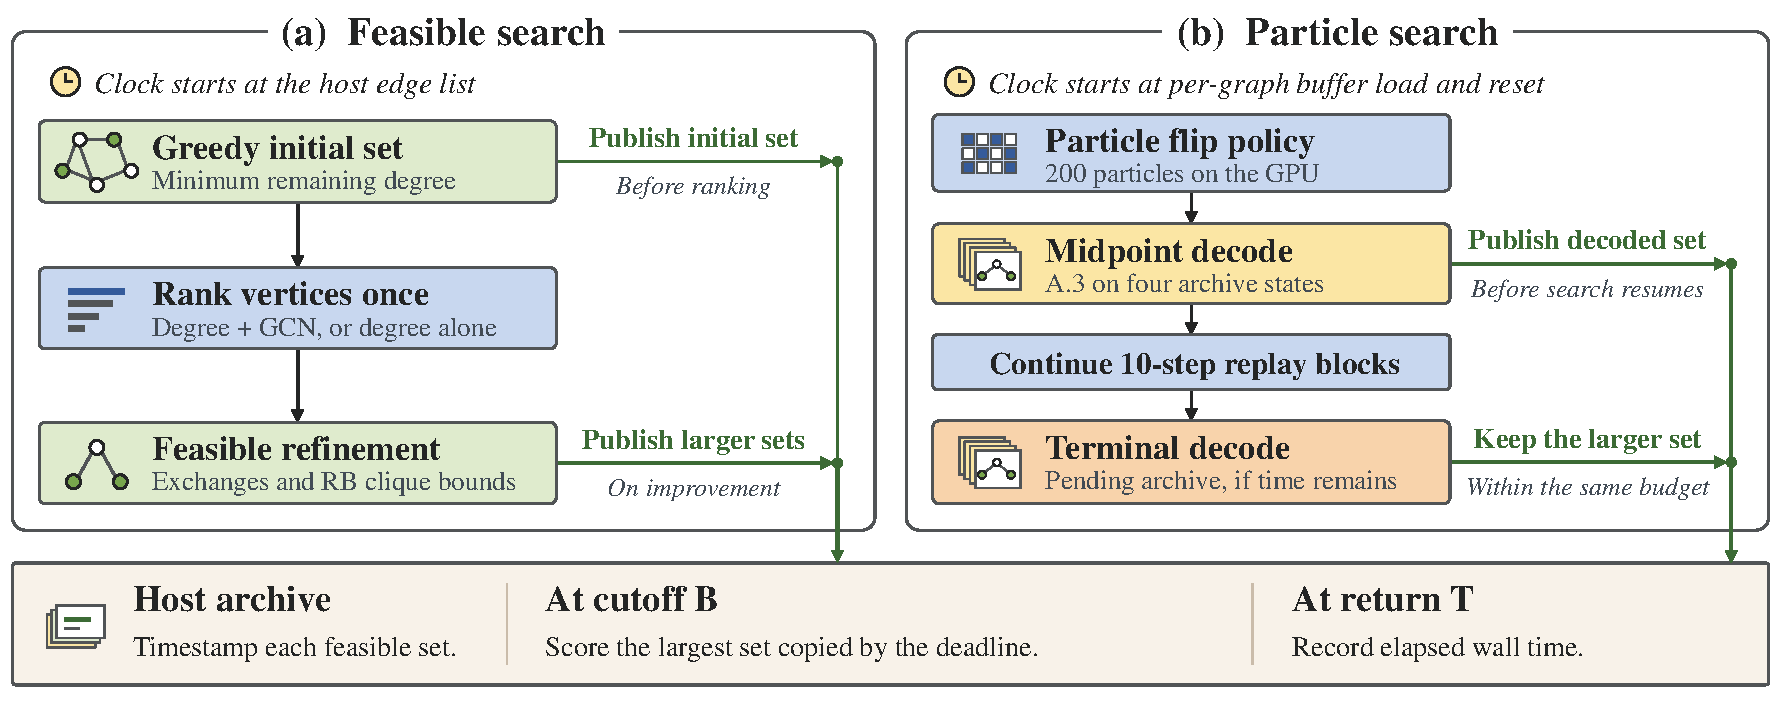
\includegraphics[width=.95\textwidth]{figures/search_paths.pdf}
\caption{\textbf{Two routes to an independent set before the deadline.} Panel titles name the routes: feasible search is SPRINT-C and particle search is SPRINT-S.
Dark arrows show execution order. Green arrows carry feasible vertex sets to the host.
(a) SPRINT-C publishes the greedy set before ranking vertices. The learned and degree-only rankings share the same refinement schedule.
(b) SPRINT-S publishes at the midpoint and again before return. Each readout decodes the four lowest-energy archive entries. Both decodes and their host copies count toward the per-graph budget.
At cutoff \(B\), the host scores the largest set it has received. The solver's return time \(T\) is recorded separately.}
\label{fig:search-paths}
\end{figure*}


For a graph \(G=(V,E)\), we seek the largest \(S\subseteq V\) with no edge inside \(S\). Figure~\ref{fig:search-paths} shows the two routes. SPRINT-C constructs an incumbent before running the network and then improves it. SPRINT-S explores conflicting states and pays a decode whenever it publishes an incumbent. In both designs the clock starts with the input in the representation the solver works from, and every published set is copied to a host archive with a timestamp.

\subsection{What can the host use at the cutoff?}
Let \(\tau_j\) be the elapsed time at which the vertices of a feasible set \(S_j\) have been copied to the host archive. At a deadline \(B\) we record
\begin{align}
 Q_B &= \max\bigl(\{\,|S_j|:\tau_j\leq B\,\}\cup\{0\}\bigr), \label{eq:score}\\
 C_B &= \mathbf{1}\{\,\exists j:\tau_j\le B\,\}. \label{eq:coverage}
\end{align}
A missed delivery contributes zero to the mean of \(Q_B\). On a covered run, \(t_B^*=\min\{\tau_j: |S_j|=Q_B,\ \tau_j\leq B\}\) is the earliest time the final score was readable. We also record the solve's return time \(T\): a set archived at 190~ms scores at a 200~ms cutoff even if the call returns at 205~ms. The three quantities separate what was delivered from what was computed. Comparisons pair runs on graph and search seed; for a contrast we average the per-graph differences and resample graphs (Appendix~\ref{app:protocol}). After timing, every archived set is verified against the input edges.

\subsection{The constructive route: publish before ranking}
\paragraph{Initialization and ranking.}
From the host edge list the solver builds a compressed sparse row adjacency, repeatedly adds a vertex of minimum remaining degree, and deletes its closed neighborhood, breaking ties with the search seed. When the residual graph is empty it publishes the resulting maximal independent set. The learned and degree-only arms share this initialization, so their first published set is identical and the first difference between them is the ranking.

Let \(d_v\) be the original degree and \(z_G(a)\) center and scale a vector across this graph's vertices, with a \(10^{-4}\) floor on the standard deviation. Refinement uses the priority
\begin{equation}
 p_v=z_G(-d)_v+\lambda\,z_G(g_\theta(G))_v .
 \label{eq:priority}
\end{equation}
The network \(g_\theta\) is a five-layer, width-128 graph convolutional encoder evaluated once on the GPU. A linear residual readout combines the final embedding with degree and neighborhood features. On each training graph we keep the four largest of eight OnlineMIS solutions and use a vertex's frequency across them as its soft membership target. One frozen checkpoint and \(\lambda=0.25\) serve every test set; the degree-only arm sets \(\lambda=0\) and skips the forward pass. Appendix~\ref{app:protocol} gives the training and validation criteria.

\paragraph{Feasible refinement.}
One CPU thread uses the priorities to exchange selected and unselected vertices. A one-for-two move replaces a selected vertex by two nonadjacent vertices for which it was the sole conflict. The archive keeps strict improvements. On RB instances the solver also branches over a partition into cliques: with partial solution \(P\) and \(k\) cliques still holding eligible vertices, every completion has size at most \(|P|+k\), and a branch closes when that bound cannot improve the incumbent. Small RB starts with branching, large RB starts with exchanges, and ER uses exchanges throughout; the register graphs use the frozen ER schedule. The clique phase publishes its best set on return.

\paragraph{Resident comparison.}
We run both rankings and native OnlineMIS afresh from the same host edge list at \(B\in\{50,100,200,500\}\)~ms on all four released test sets, with one CPU thread and a 3~ms return reserve. The clock includes graph conversion, search, host copies, and any GPU transfers and inference. OnlineMIS's greedy solution and subsequent best-solution updates reach the archive through an in-memory callback that copies vertices and timestamps each delivery, so the classical solver can also publish before its call returns. Library and weight loading precede each batch. Appendix~\ref{app:resident} gives branch allocations and the interleaved run order.

\subsection{The speculative route: particles and decode scheduling}
The speculative route uses the RLNN flip policy \citep{feng2025regularized}. It starts \(K=200\) binary particles from independent fair bits. At step \(t\) the policy maps the state \(x^k_t\) and the normalized adjacency with self-loops \(\widetilde A\) to vertex logits; with independent \(u^k_{v,t}\sim\mathrm{Unif}(0,1)\),
\begin{equation}
 x^k_{v,t+1}=x^k_{v,t}\ \oplus\
 \mathbf{1}\!\left\{u^k_{v,t}<\sigma(f_\theta(x^k_t,\widetilde A)_v)\right\},
 \label{eq:policy-step}
\end{equation}
where \(\oplus\) flips a bit when the indicator is one. Simultaneous flips can create conflicts. Each particle keeps its lowest-energy state; with \(c(x)=\sum_{\{u,v\}\in E}x_ux_v\) counting conflicting edges and \(s(x)=\sum_v x_v\), the archive ranks states by \(2\beta c(x)-s(x)\), which is \(\beta\) times the quadratic form of the symmetric unit-weight adjacency minus the cardinality. At a readout we decode the four lowest-energy archive entries with the released A.3 single-bit decoder, whose half-weight adjacency gives
\begin{equation}
 E_{\rm dec}(x)=\beta c(x)-s(x),\qquad \beta=1.02 .
 \label{eq:decode-energy}
\end{equation}
Removing a selected vertex with \(m\geq1\) selected neighbors changes \(E_{\rm dec}\) by \(1-\beta m<0\), and adding a conflict-free vertex lowers it by one. A one-flip local minimum is therefore a maximal independent set in exact arithmetic, which is what the decoder returns. We publish the largest decoded set.

\paragraph{Budgeting both readouts.}
The particle engine compiles the dense FP16 policy and replays ten-step CUDA Graph blocks with sparse archive-energy updates \citep{gray2019cudagraphs,ansel2024pytorch}. Its instance clock starts before filling reusable device buffers and resetting particles. Let \(\widehat h\) be the last synchronized block duration, and let \(r=\max(5\,\mathrm{ms},2\widehat d)\) be a decode reserve estimated from the latest decode time \(\widehat d\), taken from warm-up for the first graph. At elapsed time \(t\) we launch another block only when
\begin{equation}
 t+\widehat h+r<B .
 \label{eq:launch}
\end{equation}
The first block boundary at or after half the wall-clock budget triggers a readout, after which we raise \(r\) from the observed decode. A terminal readout decodes any pending archive if time remains; a late terminal copy leaves a timely midpoint incumbent in place. Comparing this schedule with terminal-only decoding isolates what publishing early is worth; fixed-work against fixed-deadline runs separate block cost from the extra search that faster blocks buy.
